TODO:
\begin{itemize}
%\item Either reword Proposition 2.1 so as not to be reliant on manifolds or move to later section.
\item Fix image scalings.
\item Make note on how moving the point of action smoothly *should* vary the vector smoothly in the $(p,v)$ form...
%\item Tidy up 2.3?
\end{itemize}
\section{Vector Fields \& Constructions on Spheres}
\begin{center}
\small
\justify
\texttt{Use chapterprecishere after eventual change to memoir/book doc class.}\\
\textit{In this chapter we discuss the concept of vector fields, first in the setting of familiar Euclidean space and then specifically vector fields on spheres. We then give an explicit construction of a non-vanishing vector field on spheres of odd dimension. Finally, we give a proof due to Milnor that shows that we cannot construct such non-vanishing vector fields on spheres of an even dimension.}
\normalsize
\end{center}
\hfill\\
\texttt{Motivation/intro/note to myself:}

We will first introduce the notion of vector fields in the familiar setting of Euclidean space without venturing into the world of manifolds or vector bundles. As we shall see through the course of this chapter, a number of the important results \texttt{*key*(?)} to this \texttt{*book*(?)} can be established without the use of such machinery. In this way, we may later naturally expand and develop upon the elementary concepts and techniques first introduced in this chapter. In the second half of the chapter, we focus on the task of constructing non-vanishing vector fields on spheres.
%
%\begin{itemize}
%\item definitions
%\item examples
%\item on spheres
%\item Non-vanishing on odd
%\item Milnor proof for even
%\end{itemize}
\subsection{Vector Fields in Euclidean Space}
\texttt{Adapted from other docs:}

\noindent Vectors in Euclidean space $\mathbb{R}^n$ can be understood as either so-called ``free vectors'' in which we simply think of $\mathbb{R}^n$ as a Euclidean vector space. Alternatively, we can think of ``place-bound vectors'' at a point in $\mathbb{R}^n$, in which we consider $\mathbb{R}^n$ as a metric space, the vectors in which form the points of the space. These ``place-bound vectors'' then form vector spaces in their own right, each one consisting of all possible vectors attached to a particular point. An example of a consequence following from this train of thought is that vectors at different points cannot be added/subtracted (this is a crucial idea that will become important later when we wish to differentiate vector fields in more general spaces!).

This second concept of a vector in $\mathbb{R}^n$ leads us to the notion of the tangent space at a point in $\mathbb{R}^n$.
\begin{definition}
A \textit{tangent vector} $v_x$ to Euclidean space $\mathbb{R}^n$ consists of the pair $(x,v)$, $x\in\mathbb{R}^n$ and $v\in\mathbb{R}^n$, where $x$ is referred to as the \textit{point of action} and $v$ is a vector.
\end{definition}
Then tangent vectors can be identified as the arrow from $x$ to $x+v$. Two tangent vectors $v_p$ and $w_q$ are equal if and only if $v=w$ and $p=q$.

\begin{figure}[h!]
\centering
\begin{subfigure}[b]{0.5\textwidth}
\includegraphics[scale=0.55]{fig/chp2-fig0-a}
%\caption{A smooth `bump' function $\xi$.}
\end{subfigure}%
\begin{subfigure}[b]{0.5\textwidth}
\includegraphics[scale=0.55]{fig/chp2-fig0-b}
%\caption{A smooth `ramp' function $\rho$.}
\end{subfigure}
\caption{Different ways of thinking of vectors in $\mathbb{R}^n$.}
\label{fig:chp2-fig1-vects}
\end{figure}

\begin{figure}[h!]
\centering
\includegraphics[scale=0.55]{fig/chp2-fig0-c}
\caption{A tangent vector $v_x$ at $x$.}
\end{figure}

In almost all contexts, we will identify the tangent vector $(x,v)$ with simply the vector $v$.

\begin{definition}
The \textit{tangent space} of $\mathbb{R}^n$ at the point $x$ is the set
\[
T_x\mathbb{R}^n=\{v_x:v\in\mathbb{R}^n\}.
\]
\end{definition}
\noindent Addition and multiplication by scalars $\lambda\in\mathbb{R}$ are introduced in this set by $(x,v)+(x,w):=(x,v+w)$ and $\lambda\cdot(x,v):=(x,\lambda\cdot v)$, respectively. These operations endow each $T_x\mathbb{R}^n$ with the structure of a real $n$-dimensional vector space.

There is then also a canonical isomorphism between $T_x\mathbb{R}^n$ and $\mathbb{R}^n$ given by $v_x\mapsto v$.

Consequently, the differential of a smooth map $f$ from $\mathbb{R}^n$ to $\mathbb{R}^m$ at the point $x$, denoted by $Df_x$ can now be interpreted as a linear map $f_{*,x}$ \texttt{maybe change/check that notation...} between the corresponding tangent spaces.

\begin{definition}
A \textit{vector field} $X$, defined on an open subset $U$ of $\mathbb{R}^n$ is a vector-valued function
\[
X:U\subset\mathbb{R}^n\to\mathbb{R}^n\times\mathbb{R}^n,
\]
of the form $x\mapsto (x,X(x))$, that assigns to each point $x\in U$, a tangent vector $X(x)\in\mathbb{R}^n_x$.
\end{definition}
\noindent \texttt{Maybe tie this definition into what was said about the differential of a map before, like in Agricola \& Friedrich...?}
\noindent As with tangent vectors, we will often identify the pair $(x,X(x))$ simply with $X$ itself.
If each component of $X$ is $C^k$ continuously differentiable then we say $V$ is a $C^k$ vector field. 


\subsubsection{Examples(?)}
Examples of vector fields include...

\begin{figure}[h!]
\centering
\begin{subfigure}[b]{0.45\textwidth}
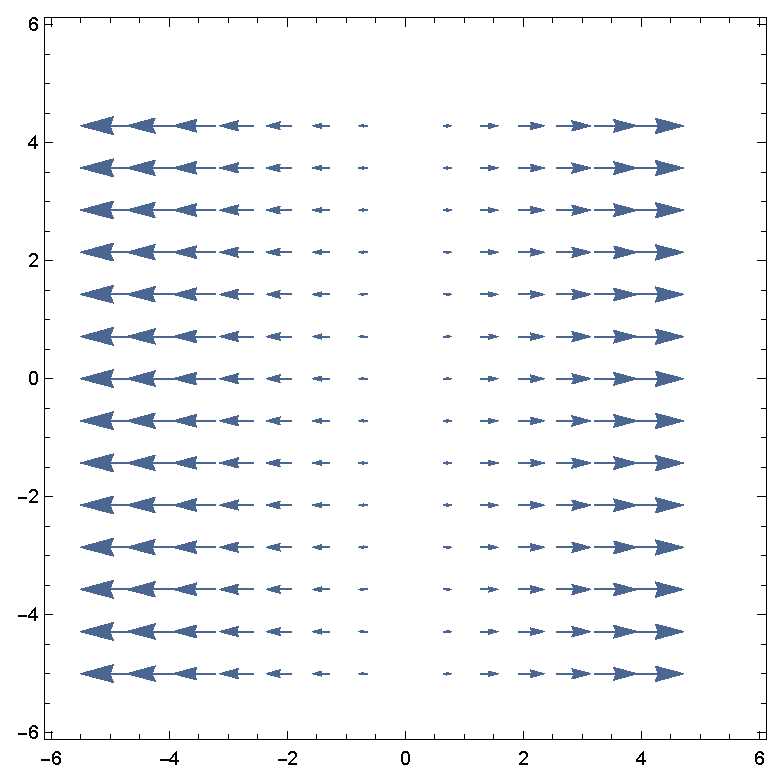
\includegraphics[scale=0.45]{fig/chp2-fig1-a}
%\caption{A smooth `bump' function $\xi$.}
\end{subfigure}%
\begin{subfigure}[b]{0.45\textwidth}
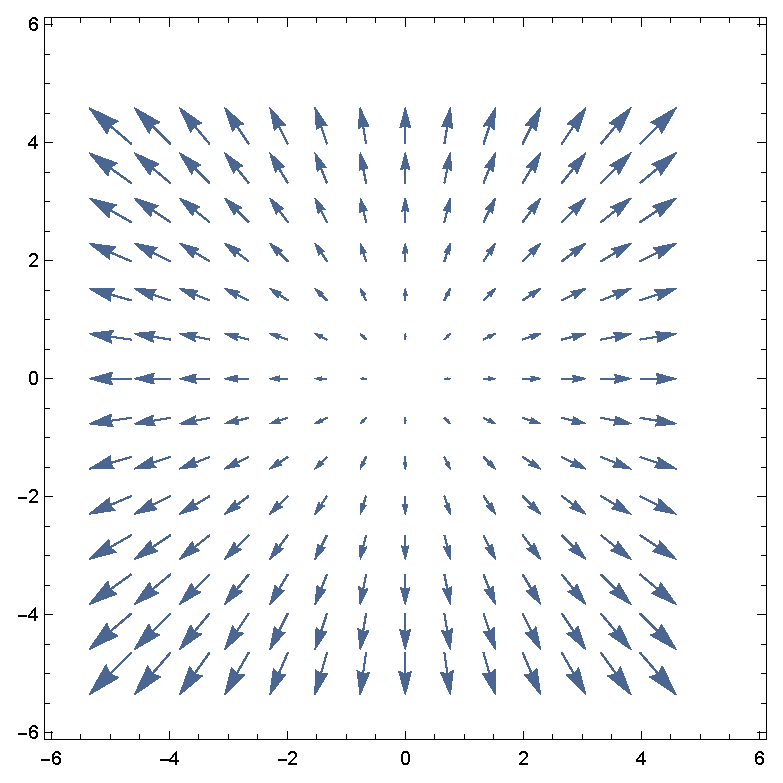
\includegraphics[scale=0.45]{fig/chp2-fig1-b}
%\caption{A smooth `ramp' function $\rho$.}
\end{subfigure}%

\begin{subfigure}[c]{0.45\textwidth}
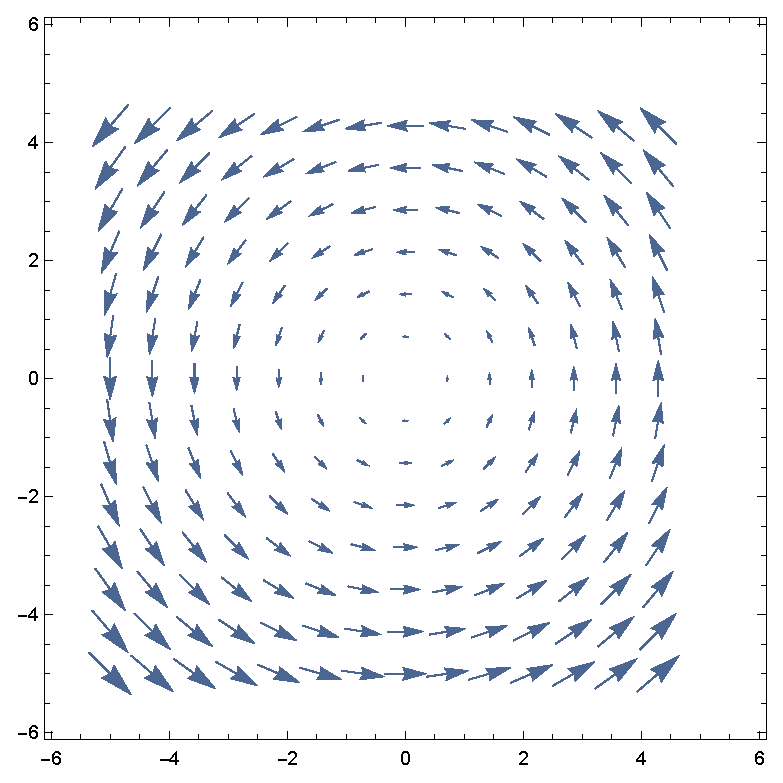
\includegraphics[scale=0.45]{fig/chp2-fig1-c}
%\caption{A smooth `ramp' function $\rho$.}
\end{subfigure}%
\begin{subfigure}[d]{0.45\textwidth}
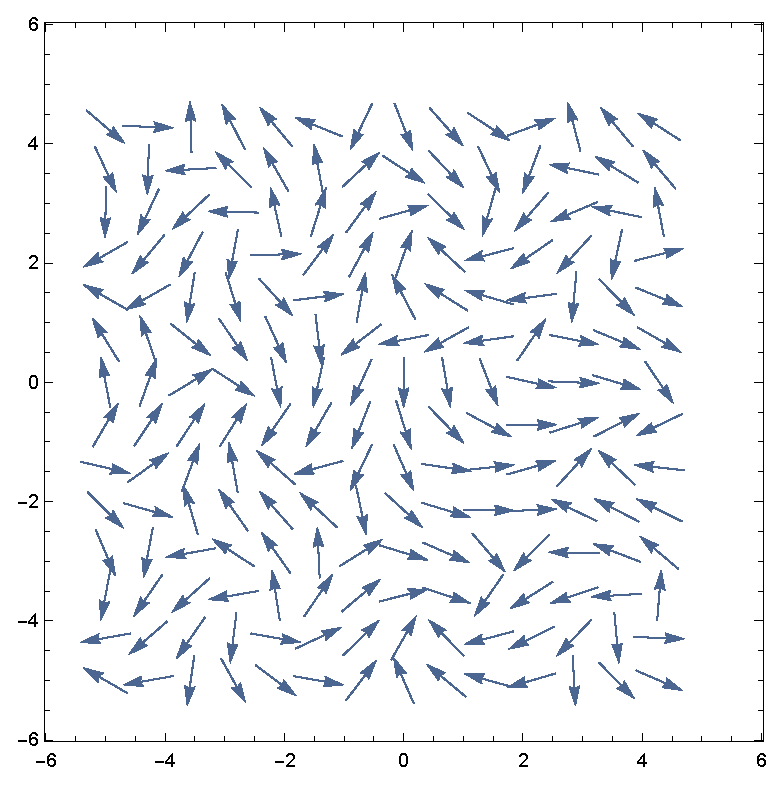
\includegraphics[scale=0.45]{fig/chp2-fig1-d}
%\caption{A smooth `ramp' function $\rho$.}
\end{subfigure}
\caption{Examples of vectors fields in $\mathbb{R}^2$.}
\label{fig:chp2-fig2-vectFields}
\end{figure}


%\begin{definition}
%Given a subset of $n$-dimensional Euclidean space, $U\subset\mathbb{R}^n$, a vector field is simply given by a vector-valued function 
%\[
%X:U\subset\mathbb{R}^n\to\mathbb{R}^n\times\mathbb{R}^n,
%\]
%of the form $x\mapsto (x,X(x))$ for $x\in\mathbb{R}^n$ and $X(x)\in\mathbb{R}^n$.
%\end{definition}

\clearpage

\noindent In coordinates we have
\[
X(x_1,\ldots,x_n)=\left(x_1,\ldots,x_n,X^1(x),\ldots,X^n(x)\right),
\]
where the $X^i(x)$ are smooth functions. Hence, then tangent vector $X(x)$ is given by
\[
X_x=\sum_iX^i(x)\left(\frac{\partial}{\partial x^i}\right)_x,
\]
which is a smoothly varying field of tangent vectors.

\noindent\texttt{From original report:}
%\begin{definition}
%If $M$ is a smooth manifold, a \textit{vector field on $M$} is a section of the tangent bundle, $X:M\to TM$. By definition of a section, if $\pi:TM\to M$ is the natural projection map of the tangent bundle, then
%\[
%\pi\circ X=\mathrm{id}_M.
%\] 
%In local coordinates we have,
%\[
%X(x_1,\ldots,x_n)=(x_1,\ldots,x_n,X^1(x),\ldots,X^n(x)),
%\]
%where the $X^i(x)$ are smooth functions. Hence the tangent vector $X(x)$ is given by,
%\begin{equation}
%X_x=\sum_iX^i(x)\left(\frac{\partial}{\partial x^i}\right)_x,
%\label{eq:vect-local}
%\end{equation}
%which is a smoothly varying field of tangent vectors.
%\end{definition}

From our definition of tangent vectors in terms of derivations, we also have the following proposition which allows us to describe vector fields in terms of derivations.
\begin{proposition}
Let $X:C^{\infty}(\mathbb{R}^n)\to C^{\infty}(\mathbb{R}^n)$ be a linear map which satisfies the Leibniz identity,
\[
X(fg)=f(Xg)+g(Xf).
\]
Then $X$ is a vector field.
\end{proposition}
\texttt{I just realised as I was re-wording this section that perhaps we should move/postpone this proposition until bundles have been established, since the proof mentions the tangent bundle and as it stands I've just gone through and replaced all instances of $M$ with $\mathbb{R}^n$ - maybe a little ``unmotivated'' or irrelevant at this point...}
\begin{proof}
Given such a derivation $X$ and $x\in M$, the map $X_x:C^{\infty}(\mathbb{R}^n)\to\mathbb{R}$ given by $X_x(f)=(X(f))(x)$ is a derivation at $x$ and so defines an element of $T_x\mathbb{R}^n$. The map $x\mapsto X_x$ from $\mathbb{R}^n$ to $T\mathbb{R}^n$ is hence a vector field and it remains to check smoothness. The components of $X_x$ with respect to the coordinate tangent basis $\partial_1,\ldots,\partial_n$ for a chart $\varphi:U\to V$ is given by,
\[
X_x^i=X_x(\varphi^i),
\]
which is by assumption a smooth function of $x$ for each $i$ (since $\varphi^i$ is a smooth function and $V$ maps smooth functions to smooth functions). We can extend the $\varphi^i$ by a bump function such as the one given by Equation \eqref{eq:bumpf-1} in a coordinate neighbourhood to convert it to a smooth function on the whole of $M$. Hence the vector field is smooth.

Conversely, given a smooth vector field $x\mapsto X_x\in T_x\mathbb{R}^n$, the map,
\[
(X(f))(x)=X_x(f),
\] 
satisfies the conditions necessary for a derivation and takes a smooth function to a smooth function.
%For all $x\in M$, $X_x(f)$ satisfies the conditions for a tangent vector at $x$, and so $X$ defines a map $X:M\to TM$ with $\pi\circ X=\mathrm{id}_M$ and can be written locally in the form of Equation \eqref{eq:vect-local}.
%
%It suffices to show that the $y_i(x)$ are smooth, and for this we simply need to apply $X$ to a coordinate function $x_i$ extended by a bump function \texttt{should probably define this earlier on somewhere eh?} in a coordinate neighbourhood. This is simply,
%\[
%Xx_i=y_i(x),
%\]
%and since by assumption $X$ maps smooth functions to smooth functions, the $y_i(x)$ are smooth.
\end{proof}

\subsection{Vector Fields on Spheres}
It suffices for now to consider the sphere $\mathbb{S}^n$ of radius $r$ in terms of an embedding in $\mathbb{R}^{n+1}$, defined by the set of points that are of distance $r$ from some central point (which we will often simply take to be the origin),
\[
\mathbb{S}^n=\left\{x\in\mathbb{R}^{n+1}:\|x\|=r\right\}.
\] 
In this manner, it follows that a vector field $X$, on the sphere $\mathbb{S}^n$ is simply a vector field in $\mathbb{R}^{n+1}$ such that
\[
x\cdot X(x)=0,\quad \forall x\in\mathbb{S}^n.
\]
In other words, for each vector $x$ on the sphere, $X$ assigns a vector $X(x)$ tangent to $\mathbb{S}^n$ at $x$.
\hfill\\

%\begin{remark}
\noindent In this work, we are interested in \textit{nowhere vanishing} vector fields on spheres. By this, it is meant that given some vector field $X$ on $\mathbb{S}^n$, we want $X(x)\neq 0$ for any given point $x\in\mathbb{S}^n$.

Given $r$ such fields $X_1,\ldots,X_r$, we will say that they are linearly independent if the vectors $X_1(x),\ldots,X_r(x)$ are linearly independent for all $x$. The central problem under investigation can then be put as follows: for each $n\in\mathbb{N}$, what is the maximum number $r$ of linearly independent vector fields on $\mathbb{S}^{n-1}$?
%\end{remark}

%\subsection{Examples}
%asdf

\subsection{Vector Field Constructions}
asdf
We have the following more general result (which also immediately implies the Hairy Ball Theorem).
\begin{theorem}
\label{thm:novan-iff-odd}
The sphere $\mathbb{S}^n$ admits an everywhere non-zero smooth vector field if and only if $n$ is odd.
\end{theorem}
In order to prove this result, we will break the theorem up into two parts. Proposition \ref{prop:even-noVF} will give the necessary condition and then in Section 3.2 we will provide the sufficient condition for the theorem.
\begin{proposition}
\label{prop:even-noVF}
If $n$ is even, then there exists no nowhere vanishing smooth vector field on $\mathbb{S}^n$.
\end{proposition}
The following proof is due to Milnor \cite{MR505523} and uses only basic techniques from analysis as opposed to other proofs that make use of more algebraic methods such as (co)homology theory.
\begin{proof}
Suppose for the sake of a contradiction, that such a vector field $V:\mathbb{S}^n\to\mathbb{R}^{n+1}$ exists. Without loss of generality, we may set $\|V(x)\|=1$ for all $x$, otherwise we may simply normalise the vector since by hypothesis $\|V(x)\|\neq 0$. Let $A$ be a compact region of $\mathbb{R}^{n+1}$ given by,
\[
A=\{y\in\mathbb{R}^{n+1}:1-\varepsilon\leq\|y\|\leq 1+\varepsilon\},
\] 
for $0<\varepsilon<1$. We can expand $V$ onto $A$ by continuing linearly over the rays, i.e. set $V(x)=\|x\|V(\frac{x}{\|x\|})$. Now consider the function,
\[
f_t(x)=x+tV(x),
\]
for $t\in\mathbb{R}$ and which is defined for all $x\in A$. Furthermore, since $\langle x,V(x)\rangle=0$ for all $x\in A$, we have that $\|f_t(x)\|=\|x\|\sqrt{1+t^2}$.

We now have the following lemmas which will give us the contradiction we seek.
\begin{lemma}
For sufficiently small $t>0$, the mapping $f_t$ is one-to-one and maps the region $A$ onto a region $f_t(A)$ whose volume can be expressed as a polynomial function in $t$.
\end{lemma}
\begin{proof}
Since $A$ is compact and since $V$ is smooth, there exists a Lipschitz constant $c>0$ such that,
\[
\|V(x)-V(y)\|\leq c\|x-y\|,
\]
for all $x,y\in A$. We see this from the fact that since all the partial derivatives are continuous, by the mean value theorem from calculus, they attain a maximum on $A$ and taking the maximum of these yields $c$.

Choose $t$ such that $|t|<c^{-1}$ and suppose that $f_t(x)=f_t(y)$. Then we get $x-y=t(V(y)-V(x))$ and hence \[\|x-y\|=|t|\|V(y)-V(x)\|\leq c|t|\|x-y\|,\] and since $0<|t|c<1$, we have that $x=y$ and so $f_t$ is injective.\\

Via the change of variables theorem, we have that,
\[
\mathrm{vol}(f_t(A))=\int_{f_t(A)}1\,\mathrm{d}y=\int_A|\mathrm{det}(Df_t(x))|\,\mathrm{d}x.
\]
We note that since $Df_t(x)=I+tD\,V(x)$ (where $I$ is the identity matrix) and the determinant of a finite dimensional matrix is a polynomial in its entries, we get that \[\mathrm{det}(Df_t(x))=1+t\sigma_1(x)+\ldots+t^k\sigma_k(x),\] where the $\sigma_i$ are polynomials of all the partial derivatives of $V$ and hence continuous in $x$. Now, choosing $t$ sufficiently small, we have that $\mathrm{det}(Df_t(x))>0$ for all $x\in A$ and we have,
\begin{align*}
\mathrm{vol}(f_t(A))&=\int_A|\mathrm{det}(Df_t(x))|\,\mathrm{d}x\\
&=\int_A\mathrm{det}(Df_t(x))\,\mathrm{d}x\\
&=\int_A\sum_{i=0}^kt^i\sigma_i(x)\,\mathrm{d}x\\
&=\sum_{i=0}^kt^k\left[\int_A\sigma_i(x)\,\mathrm{d}x\right],
\end{align*}
which is clearly a polynomial function in $t$. This completes the proof of the lemma.
\end{proof}
\begin{lemma}
For sufficiently small $t>0$, the unit sphere is mapped onto the sphere of radius $\sqrt{1+t^2}$.
\end{lemma}
\begin{proof}
When $t$ is sufficiently small, such that the determinant of $Df_t(x)$ is always strictly positive and hence $Df_t(x)$ is non-singular, we have via the inverse function theorem that $f_t$ maps open sets to open sets. As such, if we restrict $f_t$ from $\mathbb{S}^n$ to the ball $B^{n+1}$ of radius $\sqrt{1+t^2}$, we have that $f_t(\mathbb{S}^n)$ is open in the larger sphere. On the other hand, since we are working in a finite dimension, $\mathbb{S}^n$ is compact and so we have that the image under $f_t$ is also compact and hence closed in the larger sphere. Since the codomain is connected, we have that the image is both open and closed in the codomain, and so it must be the entire sphere, i.e. $f_t(\mathbb{S}^n)=B^{n+1}_{\sqrt{1+t^2}}$ and the result follows. 
\end{proof}
By the second lemma, we get that $A$ is mapped onto $\{\sqrt{1+t^2}(1-\varepsilon)\leq\|x\|\leq\sqrt{1+t^2}(1+\varepsilon)\}$, which has volume $\sqrt{1+t^2}^{n+1}\mathrm{vol}(A)$. If $n$ is even, then $\sqrt{1+t^2}^{n+1}$ is not a polynomial function. Hence, we get a contradiction with lemma 1 and so our original assumption that there exists a nowhere vanishing smooth vector field on $\mathbb{S}^n$ must be incorrect.
\end{proof}
As we are about to see, this motivating example of the Hairy Ball theorem is merely a special case of the following more general result, which also acts as a stepping stone to establishing which sphere admits parallelisations.\\

\subsection{Existence of a Non-Vanishing Vector Field}
As we have seen in the previous example and theorem, even dimensional spheres do not admit even a single everywhere non-zero smooth vector field. This tells us that we must focus our study solely on odd dimensional spheres. Ultimately, we wish to establish some maximal number of independent vector fields; before this however, an important question to perhaps ask, is whether there exists even one pointwise linearly independent vector field on $\mathbb{S}^n$.

The answer to this question thankfully, is ``yes'', we can guarantee the existence of at least one nowhere vanishing smooth vector field on $\mathbb{S}^n$. If $n$ is odd, writing $n=2k-1$, the sphere $\mathbb{S}^n$ can be embedded in $\mathbb{R}^{2k}$ and we can write down the following nowhere vanishing vector field $V:\mathbb{S}^{2k-1}\to\mathbb{R}^{2k}$ given by,
\begin{equation}
V(x_1,x_2,\ldots,x_{2k-1},x_{2k})=(-x_2,x_1,\ldots,-x_{2k},x_{2k-1}).
\label{eq:novan-vect-1}
\end{equation}
Clearly, any point $x$ on the sphere is not zero and so $V(x)$ is nowhere vanishing for all points $x\in\mathbb{S}^{2k-1}$.\\

Furthermore, we have,
\[
x\in\mathbb{R}^{2k}\mapsto (x,V(x))\in\mathbb{R}^{2k}\times\mathbb{R}^{2k}=T\mathbb{R}^{2k}.
\] 
Consider the position vector field on the sphere $R$ which is given by,
\[
x\mapsto (x,x),
\]
It can be shown through a tedious but simple computation that,
\[
\langle V(x),R(x)\rangle=0.
\]
This is to say then that the vector field $V$ is orthogonal $R$, but $R$ is also the normal vector field to the sphere. So $V$ must be tangent to the sphere.\\

The construction given above together with Proposition \ref{prop:even-noVF} concludes the proof for Theorem \ref{thm:novan-iff-odd}.